
El experimento tuvo como objetivo obtener la curva característica de un diodo semiconductor y, a partir de las mediciones de corriente y voltaje en polarización directa, estimar la relación entre la carga del electrón y la constante de Boltzmann, \(e/k_B\). Para ello se midió la corriente \(I_d\) que circulaba por el diodo y la diferencia de potencial \(V_d\) entre sus terminales al variar el voltaje de entrada \(V_i\). Las mediciones se realizaron tanto en polarización directa como en polarización inversa.

\subsection{Materiales}

Para el montaje experimental se utilizó una consola LEB01, un módulo M05, dos multímetros digitales, un termómetro, tres cables BNC plug-plug, seis cables banana de \(4\,\mathrm{mm}\) y un conector BNC tipo T jack-plug-jack. El módulo M05 contenía el circuito de polarización del diodo, el cual se muestra en la Figura \ref{dag_circuito}. Uno de los multímetros se empleó para medir el voltaje en el diodo, mientras que el otro se utilizó para medir la corriente que circulaba a través de él.

\begin{figure}[h]
    \centering
    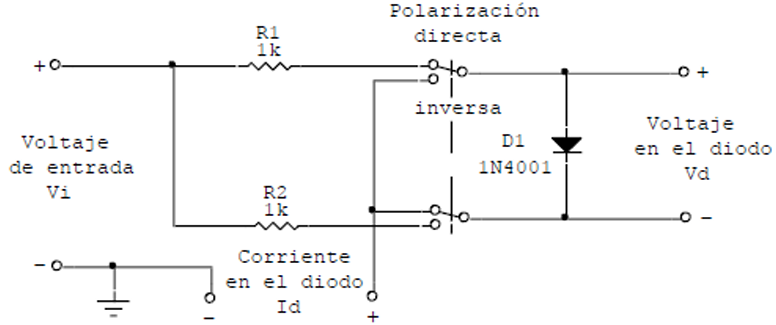
\includegraphics[width=\columnwidth]{figuras/circuito.png}
    \caption{Circuito de polarizacion del diodo}
    \label{dag_circuito}
\end{figure}

\subsection{Diseño experimental}

El módulo M05 se conectó a uno de los puertos disponibles de la consola LEB01. La fuente de voltaje variable positiva de la consola se conectó a la entrada correspondiente del módulo, cuidando la polaridad de las terminales. El circuito permitió seleccionar la polarización directa o inversa del diodo mediante el interruptor del módulo.\\

La diferencia de potencial en el diodo, \(V_d\), se midió conectando un multímetro en modo voltímetro de corriente directa entre las terminales correspondientes a los puntos \(a\) y \(b\) de la consola. La corriente del diodo, \(I_d\), se midió conectando el segundo multímetro en serie con el módulo M05, usando las terminales adecuadas para medición de corriente en la escala de miliamperes. Además, se registró la temperatura ambiente \(T\). El arreglo es el mostrado en la Figura \ref{arreglo}

\begin{figure}[h]
    \centering
    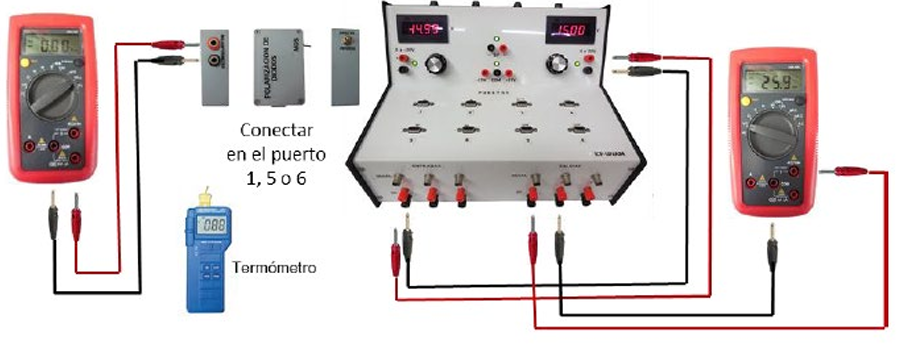
\includegraphics[width=\columnwidth]{figuras/arregloexp.png}
    \caption{Esquema de conexión.}
    \label{arreglo}
\end{figure}

La relación teórica utilizada para el análisis fue la ecuación de Shockley para polarización directa

\begin{equation}
    I_d = I_s \left[
    \exp\left(
    \frac{e V_d}{n k_B T}
    \right) - 1
    \right]
\end{equation}

donde \(I_s\) es la corriente de saturación inversa, \(e\) es la carga del electrón, \(k_B\) es la constante de Boltzmann, \(T\) es la temperatura absoluta del diodo y \(n\) es el factor de idealidad. Para corrientes suficientemente grandes $I \gg I_s$ en polarización directa, se consideró la aproximación

\begin{equation}
    I_d \simeq I_s
    \exp\left(
    \frac{e V_d}{n k_B T}
    \right)
\end{equation}

por lo que la linealización queda dada por

\begin{equation}
    \label{eqlineal}
    \ln I_d =
    \frac{e}{n k_B T} V_d + \ln I_s
\end{equation}

De esta forma, al ajustar linealmente \(\ln I_d\) como función de \(V_d\), la pendiente \(m\) permite estimar

\begin{equation}
    \frac{e}{k_B} = m n T
\end{equation}

\subsection{Procedimiento}

Primero se conectó el módulo M05 a la consola LEB01 y se verificó que las conexiones coincidieran con el esquema del circuito de polarización del diodo. Posteriormente, se conectaron las terminales de la fuente de voltaje variable positiva a la entrada del módulo mediante cables banana, cuidando que la polaridad fuera correcta.\\

Después se conectó un multímetro en modo voltímetro de corriente directa para medir la diferencia de potencial \(V_d\) entre las terminales del diodo. El segundo multímetro se configuró para medir corriente directa en la escala de miliamperes y se conectó a las terminales correspondientes del módulo M05 para registrar la corriente \(I_d\).\\

Una vez verificado el montaje, el interruptor del módulo M05 se colocó en la posición de polarización directa y se encendió la consola. Se varió el voltaje de entrada \(V_i\) desde \(0\,\mathrm{V}\) hasta \(15\,\mathrm{V}\) en pasos de $0.5V$. Para cada valor aplicado de \(V_i\), se registraron simultáneamente el voltaje en el diodo \(V_d\) y la corriente \(I_d\).\\

Posteriormente, se repitió el procedimiento colocando el interruptor del módulo en la posición de polarización inversa. En esta configuración se midieron nuevamente los valores de \(V_d\) e \(I_d\) para distintos valores del voltaje aplicado. Debido a que la corriente inversa esperada es pequeña, se cuidó que la escala del instrumento fuera adecuada para registrar variaciones pequeñas de corriente.\\

Durante el experimento, se midió la temperatura ambiente del laboratorio con el termómetro.
